%% ============================================================
%% 分片 09：原文第 4 节「Compactification And The Geometry Of Hitchin's Moduli Space」（原文 glshort.tex 起于第 2325 行）
%% 由 tools/harvmac2tex.py 从 arXiv 源码（hep-th/0604151v3）自动生成。
%% 只译英文散文；公式、编号、\label、\cite 一律不改。
%% ============================================================

\subsection{$\M_H$ 作为超凯勒商}

\label{sec:mhhyper}

对我们来说，核心重要的事实是：$\M_H$ 可以看作一个超凯勒商，因而本身就是一个超凯勒流形。我们的第一个目标就是说明这是如何产生的。

我们考虑黎曼面 $C$ 上的一个规范场论问题：其中的场是一个规范场 $ A$ 以及一个取值于伴随表示的一形式 $\phi$。（它们来自把第~\ref{sec:tqftfour}~节 中为在一般四维流形 $M$ 上构造扭化规范场论而出现的场 $A,\phi$ 限制到 $C$ 上。）我们把所有场 $A,\phi$ 构成的空间看作一个无穷维仿射空间 $\EUW$。我们用 $\delta$ 表示 $\EUW$ 上的外微分（若把它记作 $d$，就会与 $C$ 上的外微分混淆；但愿也不会与第~\ref{sec:tqftfour}~节 中用符号 $\delta_S$ 表示超对称变分相混淆）。

我们通过% 式 (4.2)
\setcounter{equation}{1}
\begin{equation}\label{eq:igob}
ds^2=-{1\over
4\pi}\int_C|d^2z|\,\Tr\left(\delta A_z\otimes \delta A_{\bar
z}+\delta A_{\bar z}\otimes \delta A_z +\delta \phi_z\otimes
\delta \phi_{\bar z}+\delta \phi_{\bar z}\otimes \delta
\phi_z\right).
\end{equation}在 $\EUW$ 上定义一个平坦度规。这里，对 $C$ 上的局部复坐标 $z$，我们写 $A=dz\,A_z+d\bar z A_{\bar z}$，$\phi = dz\,\phi_z+d\bar z\,\phi_{\bar z}$，而 $|d^2z|$ 是 $(1,1)$-形式 $i dz\wedge d\bar z$ 所对应的测度。这个 $\EUW$ 上的度规（在它之下 $\EUW$ 是无穷维欧氏空间）由 $C$ 上的复结构决定（并且不依赖于我们书写它时所用的局部坐标 $z$）。

我们希望把这个 $\EUW$ 上的平坦度规延拓为一个平坦的超凯勒结构。为此，我们在 $\EUW$ 上引入三个复结构 $I,J,$ 与 $K$，它们服从某些公理。它们都将在这仿射空间 $\EUW$ 上平移不变，因此可以由一形式空间上的（常）线性变换来定义。任何平方为 $-1$ 的线性变换都定义一个复结构；可积性是自动的。

\begin{figure}[htbp]
\centering
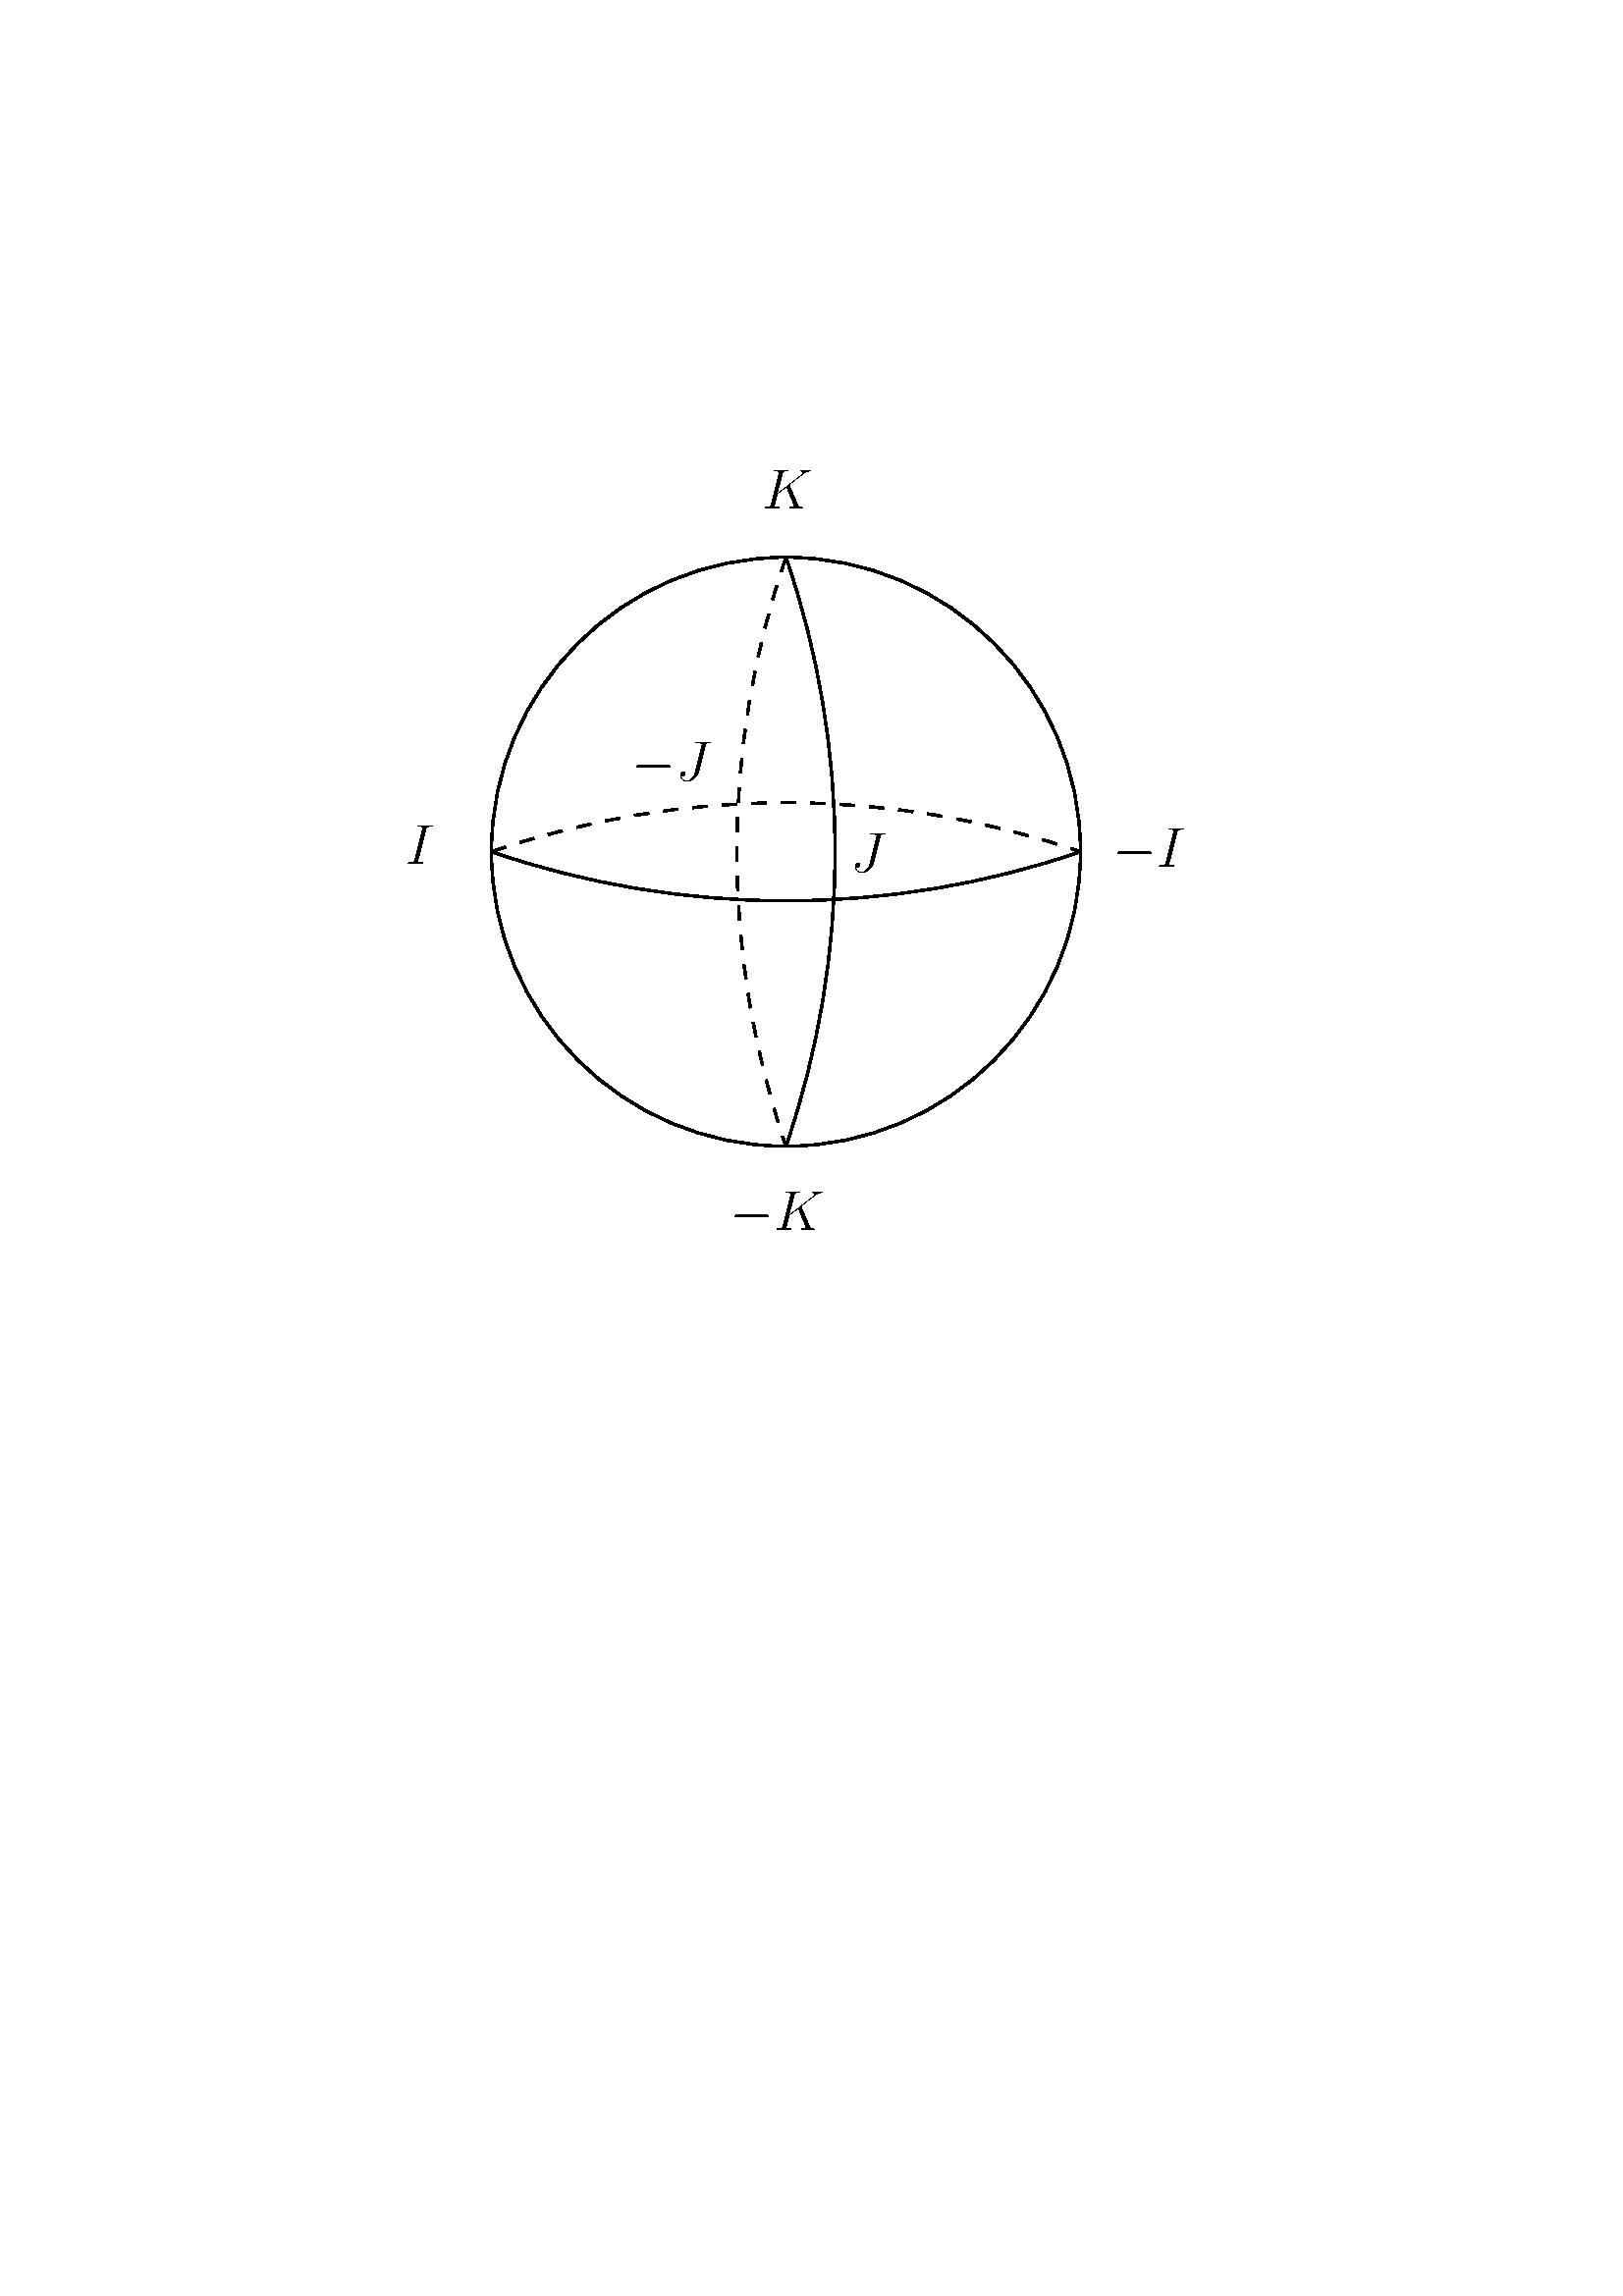
\includegraphics[width=0.75\linewidth]{figures/gla0-2.png}
\caption{ \medskip 超凯勒流形 $\M_H$ 上的一族复结构。（原文 Fig.~2）}
\label{fig:xunko}
\end{figure}
像 $I, J$ 或 $K$ 这样的复结构，通常定义为切空间上的线性变换，但我们改为写下作用在余切空间上的转置矩阵 $I^t$、$J^t$ 与 $K^t$。我们用下式定义 $I^t$% 式 (4.3)
\setcounter{equation}{2}
\begin{equation}\label{eq:uttu}
\begin{aligned} I^t(\delta A_{\bar z} )& =
i\delta A_{\bar z} \\ I^t(\delta \phi_{z}) & = i\delta \phi_{ z}
\\ I^t(\delta A_{ z}) & = -i\delta A_{ z} \\ I^t(\delta
\phi_{\bar z}) & = -i\delta \phi_{\bar z}, \\\end{aligned}
\end{equation}它们确实保证 $I^2=(I^t)^2=-1$。仿射空间 $\EUW$ 上的平移不变复结构也可以这样刻画：指明 $\EUW$ 上哪些线性函数是全纯的。对于复结构 $I$，线性全纯函数是 $A_{\bar z}$ 与 $\phi_z$（在 $C$ 上任意点取值）。

类似地，我们通过下式定义复结构 $J$：
% 式 (4.4)
\setcounter{equation}{3}
\begin{equation}\label{eq:buttu}
\begin{aligned}J^t(\delta A_{\bar z}) & = -\delta \phi_{\bar
z}\\ J^t(\delta A_z) & = -\delta \phi_z \\  J^t(\delta\phi_{\bar
z}) &  = \delta A_{\bar z} \\ J^t(\delta \phi_{ z}) & = \delta
A_z.\\\end{aligned}
\end{equation}
线性全纯函数是 $\CA_{\bar z}=A_{\bar z}+i\phi_{\bar z}$ 与 $\CA_z=A_{z}+i\phi_z$，或者更简洁地写成 $\CA=A+i\phi$。

最后，我们通过下式定义复结构 $K$：
% 式 (4.5)
\setcounter{equation}{4}
\begin{equation}\label{eq:bluttu}
\begin{aligned}K^t(\delta A_{\bar z} )& = -
i\delta\phi_{\bar z} \\ K^t(\delta \phi_{\bar z}) & = - i\delta
A_{\bar z} \\ K^t(\delta A_{ z} )& =  i\delta\phi_{ z} \\
K^t(\delta \phi_{ z}) & = i\delta A_{ z}. \\\end{aligned}
\end{equation}
线性全纯函数是 $A_{\bar z}-\phi_{\bar z}$ 与 $A_z+\phi_z$。

这些 $\EUW$ 余切空间上的线性变换满足 $I^tJ^t=-J^tI^t=-K^t$ 及其循环置换。取转置，我们就得到四元数关系的通常形式 $IJ=-JI=K$，等等。

除四元数关系之外，超凯勒结构的定义还要求度规 $ds^2$ 在每一个复结构下都是 $(1,1)$ 型。等价地，我们希望 $ds^2=I^t\otimes I^t(ds^2)=J^t\otimes J^t(ds^2)=K^t\otimes K^t(ds^2).$ 这一点可以直接验证。由于 $\EUW$ 是仿射空间且我们的复结构是线性的，没有别的东西需要检查；我们已经得到 $\EUW$ 上的一个平坦超凯勒结构。

一个超凯勒流形有（\xunko）由 $\Bbb{CP}^1$ 参数化的一族复结构，它们是 $I$、$J$ 与 $K$ 的线性组合。在我们所考虑的情形中，可以很简单地描述这族结构。对任意 $w\in \Bbb{C}^*$，我们考虑复结构 $I_w$，在其中 $A_{\bar z}-w\phi_{\bar z}$ 与 $A_z+w^{-1}\phi_z$ 全纯。于是 $w=-i$ 对应复结构 $J$，$w=1$ 对应 $K$。我们把定义延拓到包含 $w=0,\infty$：置 $I_0=I$，$I_\infty=-I$（这里 $-I$ 是与 $I$ 相反的复结构，其中 $A_z$ 与 $\phi_{\bar z}$ 全纯），因为它们是 $I_w$ 在 $w\to 0,\infty$ 时的极限。这样我们就得到所期望的那族复结构，它由一份 $\Bbb{CP}^1$ 参数化，我们把它记作 $\Bbb{CP}^1_h$（见 \zunko）。$I_w$ 的显式为
% 式 (4.6)
\setcounter{equation}{5}
\begin{equation}\label{eq:wyre}
I_w={1-\bar w w\over 1+\bar w w}I+{i(w-\bar w)\over
1+\bar w w}J+{w+\bar w\over 1+\bar w w}K.
\end{equation}
当然，它具有 $aI+bJ+cK$ 的形式，其中 $a^2+b^2+c^2=1$。

\providecommand{\CU}{{\cal U}}
我们引入一个群 $\CU_1\cong U(1)$，它按 $\phi_z\to \lambda\phi_z$、$\phi_{\bar z}\to \lambda^{-1}\phi_{\bar z}$（$|\lambda|=1$）作用于 $\phi$，同时保持 $A$ 固定。$\CU_1$ 保持超凯勒度规，并按下式作用于 $\Bbb{CP}^1_h$：% 式 (4.7)
\setcounter{equation}{6}
\begin{equation}\label{eq:zungo}
I_w\to I_{\lambda^{-1}w};
\end{equation}

它使两个点 $w=0,\infty$ 保持不动。我们在第~\ref{sec:complexstr}~节 末尾说明，$\CU_1$ 的作用在什么意义上延拓为其复化 $\CU\cong \Bbb{C}^*$ 的作用。

这族中 $\EUW$ 上的大多数复结构依赖于 $C$ 的复结构。例外的是 $J$——它可以刻画为使得 $\CA=A+i\phi$ 全纯的复结构——以及 $-J$，在其中 $\bar\CA=A-i\phi$ 全纯。$\EUW$ 上其余的复结构对 $A$ 与 $\phi$ 的 $z$ 分量与 $\bar z$ 分量区别对待，而这种区分依赖于 $C$ 的复结构。

对称群 ${\cal U}_1$ 是否来自四维杨--米尔斯理论的对称性？这个问题的答案稍微微妙。扭化的 ${\EUN}=4$ 超对称杨--米尔斯理论紧化到 $C$ 上后确实具有对称群 $\CU_1$。它通过旋转 $\phi_2-\phi_3$ 平面来作用；这是 $SU(4)_{\cal R}$ 的一个子群，在此特定紧化中未被破坏。然而，这并不给出底层那族四维拓扑场论的对称性，因为它不保持那族超对称生成元 $\epsilon=u\epsilon_\ell+v\epsilon_\rr$（它把这族生成元映到一个更大的族，我们在第~\ref{sec:twistedtft}~节 中讨论其解释，这些超对称缺少完整的 $Spin'(4)$ 对称性）。

但元素 $-1\in {\cal U}_1$ 确实来自四维拓扑场论的对称性。这个元素在 $\MH$ 上的作用，就像我们在第~\ref{sec:reviewsd}~节 中引入的中心元素 ${\EUI}\in SU(4)_{\cal R}$ 那样。事实上，${\EUI}$ 在 $SU(4)_{{\cal R}}$ 的 ${\bf 4}$ 中作用为 $i$，因此它在 ${\bf 6}=\wedge^2{\bf 4}$ 上作用为 $-1$，而后者正是包含 $\phi$ 的表示。（注意 ${\EUI}$ 也反转未扭化标量的符号。）变换 $\phi\to-\phi$ 在复结构 $I$ 下全纯，但在结构 $J$ 与 $K$ 下反全纯。这个变换的不动点集的显然分支由 $\phi=0$ 定义（正如我们后面讨论的，这给出稳定丛模空间 $\M$ 到 $\MH$ 的一个嵌入）。还有 \cite{ref20} 其他不动点集分支，在其中 $\phi$ 与 $-\phi$ 规范等价。

\par\medskip{\it 辛结构}

与 $\EUW$ 上超凯勒结构相联系的三个辛结构可定义为 $\omega_I = I^t\otimes 1(ds^2)$，类似地 $\omega_J=J^t\otimes 1(ds^2)$ 与 $\omega_K=K^t\otimes 1(ds^2)$。我们得到% 式 (4.8)
\setcounter{equation}{7}
\begin{equation}\label{eq:tomog}
\begin{aligned}\omega_I
& = -{i\over 2\pi}\int_C|d^2z|\,\Tr\left(\delta A_{\bar z}\wedge
\delta A_z-\delta \phi_{\bar z}\wedge \delta\phi_z\right)\\
&=-{1\over 4\pi}\int_C\,\Tr\left(\delta A\wedge \delta A
-\delta\phi\wedge\delta \phi\right) \\
                      \omega_J & ={1\over 2\pi}\int_C |d^2z|\,\Tr\left(
                      \delta\phi_{\bar z}\wedge \delta A_z+\delta\phi_z\wedge
                      \delta A_{\bar z} \right)\\
                      \omega_K & =
                      {i\over 2\pi}\int_C|d^2z|\,\Tr\left(\delta\phi_{\bar z}
                      \wedge\delta A_z-\delta\phi_z\wedge\delta A_{\bar z}\right)\\
                      & = {1\over 2\pi}\int_C \,\Tr\,\delta\phi
                      \wedge\delta A.\\\end{aligned}
\end{equation}

这里，$\omega_J$ 依赖于 $C$ 的复结构，而 $\omega_I$ 与 $\omega_K$ 不依赖。

此外，$\omega_I$ 关于复结构 $I$ 是 $(1,1)$ 型，$\omega_J$ 与 $\omega_K$ 也类似。我们还定义 $\Omega_I=\omega_J+i\omega_K$，以及循环置换 $\Omega_J=\omega_K+i\omega_I$、$\Omega_K=\omega_I+i\omega_J$：
 % 式 (4.9)
\setcounter{equation}{8}
\begin{equation}\label{eq:ninto}
\begin{aligned}\Omega_I & =
{1\over \pi}\int_C|d^2z|\,\Tr\,\delta\phi_z\wedge \delta A_{\bar
z} \\
        \Omega_J & =-{i\over 4\pi}\int_C\,\Tr\,\delta \CA\wedge\delta \CA          \\
        \Omega_K & = -{i\over 2\pi}\int_C |d^2z|\,\Tr\,\left( \delta A_{\bar z}\wedge
\delta A_z-\delta \phi_{\bar z}\wedge \delta\phi_z -
\delta\phi_{\bar z}\wedge \delta A_z-\delta\phi_z\wedge
                      \delta A_{\bar z}\right).\\\end{aligned}
\end{equation}

$\Omega_I$ 在复结构 $I$ 下是 $(2,0)$ 型，类似地 $\Omega_J$ 与 $\Omega_K$ 在各自的复结构下也是 $(2,0)$ 型。$\Omega_I$ 与 $\Omega_K$ 依赖于 $C$ 的复结构，但 $\Omega_J$ 不依赖。

闭二形式 $\omega_J$ 与 $\omega_K$ 实际上是恰当的。确实，我们可以非常显式地写出 $\omega_J=\delta\lambda_J$，其中 $\lambda_J={1\over 2\pi}\int_C |d^2z|\,\Tr\,\left(\phi_{\bar z}\delta A_z+\phi_z\delta A_{\bar z}\right)$。$\lambda_J$ 是规范不变的，因为 $\phi$ 与 $\delta A$（不同于 $A$ 本身）都在 $G$ 的伴随表示中变换。类似地 $\omega_K=\delta\lambda_K$，其中 $\lambda_K={1\over 2\pi}\int_C\,\Tr\,\phi\wedge \delta A$。除其他事项外，这意味着 $\MH$ 上的一个拓扑平凡线丛可以被赋予一个联络，其曲率是 $\omega_J$ 与 $\omega_K$ 的任意所需线性组合。只需把该联络取为 $\lambda_J$ 与 $\lambda_K$ 的适当线性组合即可。

另一方面，$\omega_I$ 在拓扑上非平凡。要按上面的方式写出 $\omega_I=\delta\lambda_I$，就需要在 $\lambda_I$ 中包含一个正比于 $\int \Tr \,A\wedge \delta A$ 的项，但由于 $A$ 在规范变换下的非齐次变换，这一项不是规范不变的。不过，我们可以写 $\omega_I=\omega_I'+\delta\lambda_I$，其中 $\lambda_I=(1/4\pi)\int_C\Tr\,\phi\wedge\delta\phi$，而
% 式 (4.10)
\setcounter{equation}{9}
\begin{equation}\label{eq:frox}
\omega_I'=-{1\over 4\pi}\int_C\Tr\,\delta A\wedge\delta
A.
\end{equation}
于是 $\omega_I$ 与 $\omega_I'$ 上同调，且特别地 $\omega_I$ 的上同调类是从 $\phi=0$ 的子空间拉回得到的。对单连通的 $G$，$\M$ 上线丛的 Picard 群是 $\Bbb{Z}$，由一个线丛 ${{\frak L}}$ 生成，其第一 Chern 类在 de Rham 上同调中由 $\omega_I'/2\pi$ 代表。我们会不严格地把 ${{\frak L}}$ 称作行列式线丛，因为对经典 $G$，它可以定义为 \cite{ref60} 一个 $\bar\partial$ 算子的行列式。\footnote{对 $G=SU(N)$，若 $E\to C$ 是秩为 $N$ 的全纯向量丛，则行列式线丛 $\frak L$ 在 $E$ 处的纤维 ${\frak L}_E$ 为 ${\frak L}_E=\det\,H^0(C,E)^{-1}\otimes \det\, H^1(C,E)$，其中 $\det\,V$ 表示向量空间 $V$ 的最高外幂。如此定义的线丛 $\frak L\to \M$ 是丰沛的。有些作者把我们称为 $\frak L$ 的东西写作 ${\frak L}^{-1}$。}

\par\medskip{\it Hitchin 模空间作为超凯勒商}

现在我们考虑按显然方式作用于 $\EUW$ 的规范变换群。它显然保持度规 \eqref{eq:igob}\ 与三个辛结构 \eqref{eq:tomog}。一个简短的计算表明，Hitchin 方程 \eqref{eq:zongo}\ 等价于对应于辛结构 \eqref{eq:tomog} 的三个 moment map 的消失。具体地说，设 $\epsilon$ 生成一个无穷小规范变换（因此 $\epsilon$ 是取值于 ${\rm ad}(E)$ 的零形式），并设 $V(\epsilon)$ 是 $\EUW$ 上相应的向量场，它按 $\delta A=-D\epsilon$、$\delta\phi=[\epsilon,\phi]$ 作用。那么辛结构 $\omega$ 的 moment map $\mu$ 通过解条件 $\iota_{V(\epsilon)}\omega=\delta\mu$ 得到（这里 $\iota_{V(\epsilon)}$ 是与 $V(\epsilon)$ 缩并的算子）。取 $\omega$ 为 $\omega_I$、$\omega_J$ 或 $\omega_K$，相应的 moment map 为
% 式 (4.11)
\setcounter{equation}{10}
\begin{equation}\label{eq:joget}
\begin{aligned}\mu_I & =-{1\over
2\pi}\int_C\,\Tr\,\epsilon(F-\phi\wedge \phi),\\ \mu_J &
=-{1\over 2\pi}\int_C|d^2z|\,\Tr\,\epsilon\left(D_z\phi_{\bar
z}+D_{\bar z}\phi_z\right), \\ \mu_K& = -{i\over
2\pi}\int_C|d^2z|\,\Tr\,\epsilon\left(D_z\phi_{\bar z}-D_{\bar
z}\phi_z\right).\\\end{aligned}
\end{equation}
一般地，若 $X$ 是一个超凯勒流形，李群 $H$ 以 moment map $\vec\mu=(\mu_I,\mu_J,\mu_K)$ 作用于其上，则方程 $\vec\mu=0$ 的解集对 $H$ 的商是超凯勒流形 \cite{ref61}，称为 $X$ 对 $H$ 的超凯勒商 $X/\negthinspace/\negthinspace/H$。因此特别地，$\M_H$ 是无穷维空间 ${\EUW}$ 对规范变换群的超凯勒商，并且是一个超凯勒流形。

可以给出一个更「物理」的解释，说明为什么 sigma 模型的靶空间是 $\EUW$ 的超凯勒商。一般地，在具有 $(4,4)$ 超对称与规范群 $H$ 的二维规范场论中，超多重态参数化一个超凯勒流形 $X$，而低能物理（为简单起见假设 $H$ 自由作用于 $X$）是一个 sigma 模型，其靶空间为超凯勒商 $X/\negthinspace/\negthinspace/H$。（超凯勒商构造最初正是在这一背景下被发现的 \cite{ref61}。）在目前的例子中，把四维扭化拓扑规范场论紧化到二维，得到的就是一个具有 $(4,4)$ 超对称的理论。（扭化与紧化保留了原来十六个超对称中的八个，其中四个具有一种二维手征性，另外四个具有另一种。）这个二维理论的规范群是 $C$ 到 $G$ 的映射构成的群 ${\cal G}$，而超多重态参数化 $\EUW$。这正是导致 $\MH$ 作为超凯勒商出现的那套设定。所以低能物理是一个 sigma 模型，其靶空间为 $\EUW$ 的超凯勒商。

\par\medskip{\it 维数约化的更精确描述}

我们现在可以更精确地讨论从扭化四维超对称杨--米尔斯理论到靶空间为 $\MH$ 的 sigma 模型的维数约化。这样的 sigma 模型有一个度规与一个 $B$-场。我们想确定它们是什么。

我们考虑 $M=\Sigma\times C$ 上的四维超对称杨--米尔斯理论，其中 $\Sigma $ 的半径远大于 $C$ 的半径。规范场的动能是
% 式 (4.12)
\setcounter{equation}{11}
\begin{equation}\label{eq:kinen}
{{\cmmib I}}_{kin}=-{1\over 2e^2}\int_{\Sigma\times C}
|d^2y|\,|d^2z|\,\Tr\,F_{\mu\nu}F^{\mu\nu},
\end{equation}
其中 $|d^2y|$ 与 $|d^2z|$ 分别是 $\Sigma$ 与 $C$ 上的黎曼测度。这个表达式有 $(p,q)$ 型的贡献（$p+q=2$），其中 $p$ 是切于 $\Sigma$ 的指标 $\mu,\,\nu$ 的个数，$q$ 是切于 $C$ 的个数。把 $\Sigma\times C$ 上的规范场写成 $A=A_\Sigma+A_C$ 是有用的，其中 $A_\Sigma$ 切于 $\Sigma$，$A_C$ 切于 $C$。

$(0,2)$ 型的项是 $A_C$ 的势能的一部分，它使理论局域在缓变映射 $\Phi:\Sigma\to \MH$ 上。$(2,0)$ 型的项给出 $A_\Sigma$ 的动能；在 $\MH$ 的奇点之外，由于规范群被完全破坏，这些场是有质量的，可以在红外区被积掉（正如我们在第~\ref{sec:wilbranes}~节 中明确描述的）。

sigma 模型的动能来自 $(1,1)$ 型的项。这些项是% 式 (4.13)
\setcounter{equation}{12}
\begin{equation}\label{eq:binen}
-{1\over e^2}\int
|d^2y|\,|d^2z|\,\sum_{\mu=0,1}\sum_{\nu=2,3}\,\Tr\,F_{\mu\nu}F^{\mu\nu}.
\end{equation}

我们想把它与映射 $\Phi:\Sigma\to X$ 的一般 sigma 模型相比较，其中靶空间 $X$ 用局部坐标 $X^I$ 写成度规 $ds^2_X=g_{IJ}(X)\,dX^I\,dX^J$。于是 sigma 模型的动能为
% 式 (4.14)
\setcounter{equation}{13}
\begin{equation}\label{eq:zinen}
\int |d^2y|\, g_{IJ}\sum_{\mu=0,1}\partial_\mu
X^I\partial^\mu X^J.
\end{equation}
在比较 \eqref{eq:binen}\ 与 \eqref{eq:zinen}\ 时，$X^I$ 的角色由 $A_C$ 扮演，而 $F_{ij}$ 对应于 $\partial_i X^I$。如果把 \eqref{eq:binen}\ 与 \eqref{eq:zinen}\ 和我们对 ${\EUW}$ 上超凯勒度规 $ds^2$ 的原始定义 \eqref{eq:igob}\ 相比较（该度规在超凯勒商 $\MH$ 上诱导出一个我们也称为 $ds^2$ 的度规），就会看到由四维规范场论诱导的度规 $ds^2_g$ 与 $ds^2$ 的关系为% 式 (4.15)
\setcounter{equation}{14}
\begin{equation}\label{eq:inog}
ds^2_g={4\pi\over e^2}\,ds^2=({\rm
Im}\,\tau)\,ds^2.
\end{equation}

类似地，我们想约化规范场论的 $\theta$ 项，它在欧氏号差下为% 式 (4.16)
\setcounter{equation}{15}
\begin{equation}\label{eq:bloko}
{\cmmib
I}_\theta={i\theta\over 8\pi^2}\int_{\Sigma\times C}\,\Tr\,
F\wedge F.
\end{equation}
同样地，我们对代表到 $\MH$ 的缓变映射的规范场来赋值这个耦合。由于 ${{\cmmib I}}_\theta$ 的拓扑不变性，在计算 \eqref{eq:bloko}\ 时我们可以形变到 $F$ 在 $C$ 上的限制为零的情形（即 $F_{23}=0$）。形变到 $F|_C=0$ 可以通过一个复规范变换或利用 Hitchin 的第二纤维化 $\MH\to\M$ 来实现（这两个概念我们后面都会解释）。既然如此，在计算 ${\cmmib I}_\theta$ 时，我们可以把 $F={1\over 2}\sum_{\mu,\nu=0}^3dx^\mu\wedge dx^\nu \,F_{\mu\nu}$ 替换为 $F^{1,1}=\sum_{\mu=0,1}\sum_{\nu=2,3}dx^\mu\wedge dx^\nu \,F_{\mu\nu}$。在 sigma 模型极限下，$F^{1,1}$ 对应于 $\delta A_C=\sum_{\mu=0,1}dx^\mu \,D_\mu A_C$，而 ${\cmmib I}_\theta$ 约化为\footnote{出现一个负号是因为：在定义 $\omega_I'$ 时，$\delta$——即联络 $A_C$ 构成的空间上的外微分——被取为与 $C$ 上诸如 $dx^ j$（$j=2,3$）这样不依赖于 $A_C$ 的一形式交换。而对于 $\Sigma\times C$ 上的微分形式（${\cmmib I}_\theta$ 正是用它定义的），它们会反交换。}
% 式 (4.17)
\setcounter{equation}{16}
\begin{equation}\label{eq:ino}
-{i\theta\over 8\pi^2}\int_\Sigma \int_C \Tr\,\delta
A_C\wedge \delta A_C.
\end{equation}

与 $\omega_I'$ 的定义 \eqref{eq:frox}\ 相比较，我们看到这等价于% 式 (4.18)
\setcounter{equation}{17}
\begin{equation}\label{eq:zinok}
{i\theta\over
2\pi}\int_\Sigma\Phi^*(\omega'_{I})={i\theta\over 2\pi}\int_\Sigma
\Phi^*(\omega_I),
\end{equation}
其中最后一步用到了 $\omega_{I}-\omega'_{I}$ 是恰当的这一事实。在一般 sigma 模型中，$B$-场是靶空间 $X$ 上的闭二形式；它通过一项 $-i\int_\Sigma\,\Phi^*(B)$ 出现在作用量中。因此，有效低能 sigma 模型的 $B$-场为
% 式 (4.19)
\setcounter{equation}{18}
\begin{equation}\label{eq:palooka}
B=-{\theta\over 2\pi}\omega_I=-({\rm
Re}\,\tau)\,\omega_I.
\end{equation}

我们可以更概念化地描述这一点。对单连通的 $G$，瞬子数 $(1/8\pi^2)\int_M \Tr\,F\wedge F$ 对任意四维流形 $M$ 都取整数值。此外，对单连通的 $G$，$\MH$ 是单连通的，因而 $H^2(\MH,\Bbb{Z})=\pi_2(\MH)$。形式 $\omega_I$ 的归一化使得 $\omega_I/2\pi$ 是 $H^2(\MH,\Bbb{Z})$ 的一个生成元在 de Rham 上同调中的像。这些事实意味着：对任意 $\Sigma$ 与 $C$，存在映射 $\Phi:\Sigma\to \MH$ 使 $\int_\Sigma\Phi^*(\omega_I/2\pi)=1$（而且这是可达到的最小值）。这样的映射对应于 $M=\Sigma\times C$ 上一个规范场，其瞬子数按约定为 $\pm 1$。\footnote{在物理论文中，四维瞬子一般取为自对偶规范场，满足 $F^-=0$；而在数学文献中，一般取为反自对偶，满足 $F^+=0$。如果把 sigma 模型中的瞬子理解为到 $\MH$ 的全纯映射，并采用四维中通常的物理约定，那么瞬子数为 1 的 sigma 模型场来自瞬子数为 $-1$ 的规范场论瞬子。通常的数学约定避免了这一负号。}更简单地说，二维与四维中的 $\theta$ 角相同，因为瞬子是相同的。若 $G$ 不是单连通的，情况会稍复杂一些；瞬子数不总是整数，而在 sigma 模型一侧也有相应的复杂化。

\begin{yizhu}[易错点]
按：$I$ 与 $J$ 的区分是本节乃至整个 §4 的枢纽，务必记牢。复结构 $I$ 中的线性全纯函数是 $A_{\bar z}$ 与 $\phi_z$：这把 $A$ 的 $(0,1)$ 部分读作全纯丛的结构、把 $\phi$ 的 $(1,0)$ 部分读作 Higgs 场，于是 $I$ 对应「半稳定 Higgs 丛」的图像；复结构 $J$ 中的全纯函数是 $\CA=A+i\phi$，即复平坦联络，于是 $J$ 对应「平坦 $G_{\Bbb C}$ 丛」的图像（记作 $Y$，而且 $J$ 不依赖 $C$ 的复结构）；$K=IJ$ 是第三个结构。相应地把参数对应关系记住：$w=-i\leftrightarrow J$，$w=1\leftrightarrow K$，$w=0\leftrightarrow I$，$w=\infty\leftrightarrow -I$。后面讨论 $S$-对偶时交换的是 $I$ 与 $J$（A-模型与 B-模型的靶空间互换），若把这两个复结构弄混，膜与 Hitchin 纤维的对应就会全部颠倒。
\end{yizhu}

\begin{yizhu}[易错点]
按：(4.11) 的三个 moment map 方程 $\mu_I=\mu_J=\mu_K=0$ 就是 Hitchin 方程。具体地，$\mu_I=0$ 给出 $F-\phi\wedge\phi=0$；而 $\mu_J=0$ 与 $\mu_K=0$ 合起来等价于两个复方程 $D_z\phi_{\bar z}=0$ 与 $D_{\bar z}\phi_z=0$——取 $\mu_J$ 与 $\mu_K$ 的线性组合时，对称部分与反对称部分分别消去一个方向。这正是四维中 $D\phi=0$、$D\star\phi=0$ 两个实方程在二维的化身。另一个易混点是量纲：$\EUW$ 是无穷维仿射空间，$\epsilon$ 取值在 ${\rm ad}(E)$ 中，moment map 作为 $\EUW$ 上的「函数」其实取值在对偶空间（即分布）里，所以 (4.11) 中保留了 $\int_C\Tr\,\epsilon(\dots)$ 的积分形式；不要以为这是多余的记号。
\end{yizhu}

\begin{yizhu}[物理图像]
按：这一段是超凯勒商构造的原始物理背景。二维 $(4,4)$ 超对称规范理论中，超多重态的参数空间是超凯勒流形 $X$，规范群 $H$ 的作用给出超凯勒商 $X/\negthinspace/\negthinspace/H$：低能下超多重态被约束到 moment map 零点，而规范多重态有质量、被积掉。在本例中 $X=\EUW$（无穷维！）、$H={\cal G}={\rm Maps}(C,G)$，所以 $\MH=\EUW/\negthinspace/\negthinspace/{\cal G}$ 自动继承超凯勒结构。无穷维的商之所以能给出有限维流形，是因为 Hitchin 方程是椭圆方程组，其解模空间有限维；这一「无穷维商仍超凯勒」的机制正是后面所有超凯勒几何论证的基础。
\end{yizhu}

\begin{yizhu}[含糊点拨]
按：(4.15) 与 (4.19) 合起来说明二维 sigma 模型的两个连续参数恰好来自四维的规范耦合：度规由 $e^2$ 决定、$B$-场由 $\theta$ 决定。若取本书的复耦合约定 $\tau=\theta/2\pi+4\pi i/e^2$，则 ${\rm Im}\,\tau=4\pi/e^2$ 给出度规、${\rm Re}\,\tau=\theta/2\pi$ 给出 $B$-场，二者合起来正是 $\tau$。注意 $B$-场正比于 $\omega_I$（而不是 $\omega_J$ 或 $\omega_K$）：因为 $\theta$ 项的约化只留下 $\omega_I'$ 的部分，而 $\omega_I$ 与 $\omega_I'$ 上同调，故在作用量中可以互换。$B$-场不是四维理论的基本数据，而是 $\theta$ 项在紧化下的产物；话虽如此，它在二维理论中却是能灵敏感知瞬子数的数据。
\end{yizhu}

\begin{yizhu}[易错点]
按：为什么二维 sigma 模型的 $\theta$ 角与四维规范理论的 $\theta$ 角相同？关键在于 $\int_\Sigma\Phi^*(\omega_I/2\pi)=1$ 与四维瞬子数是同一个拓扑量：$\omega_I/2\pi$ 是 $H^2(\MH,\Bbb{Z})$ 生成元的 de Rham 像，故它在二维的积分是整数；而这个整数正是四维第二 Chern 数（瞬子数）在约化下的像，所以两边用同一个 $\theta$ 加权。末段脚注提醒物理与数学文献对自对偶/反自对偶的约定差一个符号，故同一个位形在两边瞬子数标号相反（$\pm 1$）；这是约定问题，并非方程不一致。
\end{yizhu}

\begin{yizhu}[含糊点拨]
按：$\omega_J,\omega_K$ 恰当而 $\omega_I$ 不恰当，这个不对称是 Hitchin 模空间几何的核心之一。$\omega_I$ 的上同调类来自 $\phi=0$ 的子空间（即稳定丛模空间 $\M$）的拉回，并由行列式线丛 $\frak L$ 的第一 Chern 类代表；$\omega_J,\omega_K$ 的恰当性则让 $\MH$ 上存在曲率为任意线性组合的联络。脚注中的行列式线丛在经典群时可用 $\bar\partial$ 算子的行列式定义，其丰沛性（ample）与稳定性及嵌入有关。另：本片用到的 harvmac 遗留宏不要展开或改名——\xunko 展开为「fig.~2」、\zunko 展开为「fig.~1」（是原文图号，不是 \verb|\ref{fig:...}|，勿替换）；$\CU$ 在此处是群 $\CU_1\cong U(1)$ 及其复化 $\CU\cong \Bbb{C}^*$，与别处把 $\CU$ 用作 Bun$_G$ 的记号不同，注意区分。
\end{yizhu}
